\section{Graphs and Graph Models}
A major publishing company has ten editors (referred to by 1, 2,\ldots, 10) in the scientific, technical and computing areas. These ten editors have a standard meeting time during the first Friday of every month and have divided themselves into seven committees to meet later in the day to discuss specific topics of interest to the company, namely, advertising, securing reviewers, contacting new potential authors, finances, used and rented copies, electronic editions and competing textbooks. This leads us to our first example.

\begin{exmp}
The ten editors have decided on the seven committees: $c_{1}$ = \{1,2,3\}, $c_{2}$ = \{1,3,4,5\}, $c_{3}$ = \{2,5,6,7\}, $c_{4}$ = \{4,7,8,9\}, $c_{5}$ = \{2,6,7\}, $c_{6}$ = \{8,9,10\}, $c_{7}$ = \{1,3,9,10\}. They have set aside three time periods for the seven committees to meet on those Fridays when all ten editors are present. Some pairs of committees cannot meet during the same period because one or two of the editors are on both committees. This situation can be modeled visually as shown in Figure 1.1.

\begin{figure}[h]
	\[G:
	\raisebox{-.5\height}
	{
		\begin{tikzpicture}[x=1.5cm, y=1.5cm]
			\foreach \i/\j in {0/1, -1/2, 5/3, 4/4, 3/5, 2/6, 1/7} {
				\setcounter{Angle}{90 + \i * 360 / 7};
				\vertex (c\j) at (\theAngle:1) [label=\theAngle:$c_{\j}$]{};
			}
			\path
				(c1) edge (c2)
				(c1) edge (c3)
				(c1) edge (c5)
				(c1) edge (c7)
				(c2) edge (c3)
				(c2) edge (c4)
				(c2) edge (c7)
				(c3) edge (c4)
				(c3) edge (c5)
				(c4) edge (c5)
				(c4) edge (c6)
				(c4) edge (c7)
				(c6) edge (c7)
			;
		\end{tikzpicture}
	}\]
	\caption{A graph}
\end{figure}

In this figure, there are seven small circles, representing the seven committees and a straight line segment is drawn between two circles if the committees they represent have at least one committee member in common. In other words, a straight line segment between two small circles (committees) tells us that these two committees should not be scheduled to meet at the same time. This gives us a picture or a "model" of the committees and the overlapping nature of their membership.
\end{exmp}

What we have drawn in Figure 1.1 is called a graph. Formally, a \bf{graph} $G$ consists of a finite nonempty set $V$ of objects called \bf{vertices} (the singular is \bf{vertex}) and a set $E$ of 2-element subsets of $V$ called \bf{edges}. The sets $V$ and $E$ are the \bf{vertex set} and \bf{edge set} of $G$, respectively. So a graph $G$ is a pair (actually an \it{ordered} pair) of two sets $V$ and $E$. For this reason, some write $G = (V,E)$. At times, it is useful to write $V(G)$ and $E(G)$ rather than $V$ and $E$ to emphasize that these are the vertex and edge sets of a particular graph $G$. Although $G$ is the common symbol to use for a graph, we also use $F$ and $H$, as well as $G'$, $G''$ and $G_{1}$, $G_{2}$, etc. Vertices are sometimes called \bf{points} or \bf{nodes} and edges are sometimes called \bf{lines}. Indeed, there are some who use the term \bf{simple graph} for what we call a graph. Two graphs $G$ and $H$ are \bf{equal} if $V(G) = V(H)$ and $E(G) = E(H)$, in which case we write $G = H$.

It is common to represent a graph by a diagram in the plane (as we did in Figure 1.1) where the vertices are represented by points (actually small circles -- open or solid) and whose edges are indicated by the presence of a line segment or curve between the two points in the plane corresponding to the appropriate vertices. The diagram itself is then also referred to as a graph. For the graph $G$ of Figure 1.1 then, the vertex set of $G$ is $V(G) = \{c_{1},c_{2},\ldots,c_{7}\}$ and the edge set of $G$ is
\begin{align*}
E(G) = &\{\{c_{1},c_{2}\},\{c_{1},c_{3}\},\{c_{1},c_{5}\},\{c_{1},c_{7}\},\{c_{2},c_{3}\},\{c_{2},c_{4}\},\{c_{2},c_{7}\},\\
&\{c_{3},c_{4}\},\{c_{3},c_{5}\},\{c_{4},c_{5}\},\{c_{4},c_{6}\},\{c_{6},c_{7}\}\}.
\end{align*}

Let's consider another situation. Have you ever encountered this sequence of integers before?
\begin{align*}
1, 1, 2, 3, 5, 8, 13, 21, 34, 55, \ldots
\end{align*}
Every integer in the sequence is the sum of the two integers immediately preceding it (except for the first two integers of course). These numbers are well known in mathematics and are called the \bf{Fibonacci numbers}. In fact, these integers occur so often that there is a journal (\it{The Fibonacci Quarterly}, frequently published \it{five} times a year!) devoted to the study of their properties. Our second example concerns these numbers.

\begin{exmp}
Consider the set $S$ = \{2,3,5,8,13,21\} of six specific Fibonacci numbers. There are some pairs of distinct integers belonging to $S$ whose sum or difference (in absolute value) also belongs to $S$, namely, \{2,3\}, \{2,5\}, \{3,5\}, \{3,8\}, \{5,8\}, \{5,13\}, \{8,13\}, \{8,21\} and \{13,21\}. There is a more visual way of identifying these pairs, namely by the graph $H$ of Figure 1.2. In this case, $V(H) = \{2,3,5,8,13,21\}$ and
\begin{align*}
E(H) = \{\{2,3\},\{2,5\},\{3,5\},\{3,8\},\{5,8\},\{5,13\},\{8,13\},\{8,21\},\{13,21\}\}.
\end{align*}
\end{exmp}

\begin{figure}[h]
	\[H:
	\raisebox{-.5\height}
	{
		\begin{tikzpicture}[x=1.5cm, y=1.5cm]
			\foreach \i/\j in {1/2, 0/3, 5/5, 4/8, 3/13, 2/21} {
				\setcounter{Angle}{\i * 360 / 6};
				\vertex (\j) at (\theAngle:1) [label=\theAngle:$\j$]{};
			}
			\path
				(2) edge (3)
				(2) edge (5)
				(3) edge (5)
				(3) edge (8)
				(5) edge (8)
				(5) edge (13)
				(8) edge (13)
				(8) edge (21)
				(13) edge (21)
			;
		\end{tikzpicture}
	}\]
	\caption{Another graph}
\end{figure}

When dealing with graphs, it is customary and simpler to represent an edge $\{u,v\}$ by $uv$ (or $vu$). If $uv$ is an edge of $G$, then $u$ and $v$ are said to be \bf{adjacent} in $G$. The number of vertices in $G$ is often called the \bf{order} of $G$, while the number of edges is its \bf{size}. Since the vertex set of every graph is nonempty, the order of every graph is at least 1. A graph with exactly one vertex is called a \bf{trivial graph}, implying that the order of a \bf{nontrivial graph} is at least 2. The graph $G$ of Figure 1.1 has order 7 and size 13, while the graph $H$ of Figure 1.2 has order 6 and size 9. We often use $n$ and $m$ for the order and size, respectively, of a graph. So, for the graph $G$ of Figure 1.1, $n = 7$ and $m = 13$; while for the graph $H$ of Figure 1.2, $n = 6$ and $m = 9$.

A graph $G$ with $V(G) = \{u,v,w,x,y\}$ and $E(G) = \{uv,uw,vw,vx,wx,xy\}$ is shown in Figure 1.3(a). There are occasions when we are interested in the structure of a graph and not in what the vertices are called. In this case, a graph is drawn without labeling its vertices. For this reason, the graph $G$ of Figure 1.3(a) is a \bf{labeled graph} and Figure 1.3(b) represents an \bf{unlabeled graph}.

\begin{figure}[h]
	\centering
	\begin{subfigure}[b]{.4\textwidth}
		\[G:
		\raisebox{-.5\height}
		{
			\begin{tikzpicture}[x=1.5cm, y=1.5cm]
				\vertex (u) at (90:1) [label=above:$u$]{};
				\vertex (v) at (162:1) [label=left:$v$]{};
				\vertex (w) at (18:1) [label=right:$w$]{};
				\vertex (x) at (234:1) [label=left:$x$]{};
				\vertex (y) at (306:1) [label=right:$y$]{};
				\path
					(u) edge (v)
					(u) edge (w)
					(v) edge (w)
					(v) edge (x)
					(w) edge (x)
					(x) edge (y)
				;
			\end{tikzpicture}
		}\]
		\caption{}
	\end{subfigure}%
	\begin{subfigure}[b]{.4\textwidth}
		\[\raisebox{-.6\height}
		{
			\begin{tikzpicture}[x=1.5cm, y=1.5cm]
				\vertex (u) at (90:1){};
				\vertex (v) at (162:1){};
				\vertex (w) at (18:1){};
				\vertex (x) at (234:1){};
				\vertex (y) at (306:1){};
				\path
					(u) edge (v)
					(u) edge (w)
					(v) edge (w)
					(v) edge (x)
					(w) edge (x)
					(x) edge (y)
				;
			\end{tikzpicture}
		}\]
		\caption{}
	\end{subfigure}
	\caption{A labeled graph and an unlabeled graph}
\end{figure}

Let us now turn to yet another situation.

\begin{exmp}
Suppose that we have two coins, one silver and one gold, placed on two of the four squares of a $2 \times 2$ checkerboard. There are twelve such configurations, shown in Figure 1.4, where the shaded coin is the gold coin.

\begin{figure}[h]
	\centering
	\captionsetup[subfigure]{labelformat=empty}
	%c1
	\begin{subfigure}[t]{.1\textwidth}
		\centering
		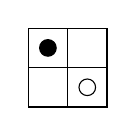
\begin{tikzpicture}[x=1cm]
			\draw (0,0)--(1,0)--(1,1)--(0,1)--cycle;
			\draw (.5,0)--(.5,.5)--(.5,1);
			\draw (0,.5)--(.5,.5)--(1,.5);
			\draw (.75,.25) circle (3pt);
			\filldraw (.25,.75) circle (3pt);
		\end{tikzpicture}
		\caption{$c_{1}$}
	\end{subfigure}%
	%c2
	\begin{subfigure}[t]{.1\textwidth}
		\centering
		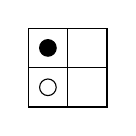
\begin{tikzpicture}[x=1cm]
			\draw (0,0)--(1,0)--(1,1)--(0,1)--cycle;
			\draw (.5,0)--(.5,.5)--(.5,1);
			\draw (0,.5)--(.5,.5)--(1,.5);
			\draw (.25,.25) circle (3pt);
			\filldraw (.25,.75) circle (3pt);
		\end{tikzpicture}
		\caption{$c_{2}$}
	\end{subfigure}%
	%c3
	\begin{subfigure}[t]{.1\textwidth}
		\centering
		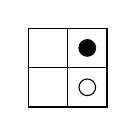
\begin{tikzpicture}[x=1cm]
			\draw (0,0)--(1,0)--(1,1)--(0,1)--cycle;
			\draw (.5,0)--(.5,.5)--(.5,1);
			\draw (0,.5)--(.5,.5)--(1,.5);
			\draw (.75,.25) circle (3pt);
			\filldraw (.75,.75) circle (3pt);
		\end{tikzpicture}
		\caption{$c_{3}$}
	\end{subfigure}%
	%c4
	\begin{subfigure}[t]{.1\textwidth}
		\centering
		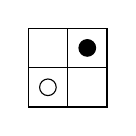
\begin{tikzpicture}[x=1cm]
			\draw (0,0)--(1,0)--(1,1)--(0,1)--cycle;
			\draw (.5,0)--(.5,.5)--(.5,1);
			\draw (0,.5)--(.5,.5)--(1,.5);
			\draw (.25,.25) circle (3pt);
			\filldraw (.75,.75) circle (3pt);
		\end{tikzpicture}
		\caption{$c_{4}$}
	\end{subfigure}%
	%c5
	\begin{subfigure}[t]{.1\textwidth}
		\centering
		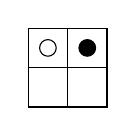
\begin{tikzpicture}[x=1cm]
			\draw (0,0)--(1,0)--(1,1)--(0,1)--cycle;
			\draw (.5,0)--(.5,.5)--(.5,1);
			\draw (0,.5)--(.5,.5)--(1,.5);
			\draw (.25,.75) circle (3pt);
			\filldraw (.75,.75) circle (3pt);
		\end{tikzpicture}
		\caption{$c_{5}$}
	\end{subfigure}%
	%c6
	\begin{subfigure}[t]{.1\textwidth}
		\centering
		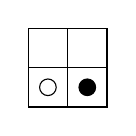
\begin{tikzpicture}[x=1cm]
			\draw (0,0)--(1,0)--(1,1)--(0,1)--cycle;
			\draw (.5,0)--(.5,.5)--(.5,1);
			\draw (0,.5)--(.5,.5)--(1,.5);
			\draw (.25,.25) circle (3pt);
			\filldraw (.75,.25) circle (3pt);
		\end{tikzpicture}
		\caption{$c_{6}$}
	\end{subfigure}
	
	%c7
	\begin{subfigure}[t]{.1\textwidth}
		\centering
		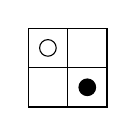
\begin{tikzpicture}[x=1cm]
			\draw (0,0)--(1,0)--(1,1)--(0,1)--cycle;
			\draw (.5,0)--(.5,.5)--(.5,1);
			\draw (0,.5)--(.5,.5)--(1,.5);
			\draw (.25,.75) circle (3pt);
			\filldraw (.75,.25) circle (3pt);
		\end{tikzpicture}
		\caption{$c_{7}$}
	\end{subfigure}%
	%c8
	\begin{subfigure}[t]{.1\textwidth}
		\centering
		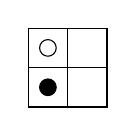
\begin{tikzpicture}[x=1cm]
			\draw (0,0)--(1,0)--(1,1)--(0,1)--cycle;
			\draw (.5,0)--(.5,.5)--(.5,1);
			\draw (0,.5)--(.5,.5)--(1,.5);
			\draw (.25,.75) circle (3pt);
			\filldraw (.25,.25) circle (3pt);
		\end{tikzpicture}
		\caption{$c_{8}$}
	\end{subfigure}%
	%c9
	\begin{subfigure}[t]{.1\textwidth}
		\centering
		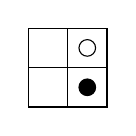
\begin{tikzpicture}[x=1cm]
			\draw (0,0)--(1,0)--(1,1)--(0,1)--cycle;
			\draw (.5,0)--(.5,.5)--(.5,1);
			\draw (0,.5)--(.5,.5)--(1,.5);
			\draw (.75,.75) circle (3pt);
			\filldraw (.75,.25) circle (3pt);
		\end{tikzpicture}
		\caption{$c_{9}$}
	\end{subfigure}%
	%c10
	\begin{subfigure}[t]{.1\textwidth}
		\centering
		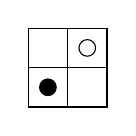
\begin{tikzpicture}[x=1cm]
			\draw (0,0)--(1,0)--(1,1)--(0,1)--cycle;
			\draw (.5,0)--(.5,.5)--(.5,1);
			\draw (0,.5)--(.5,.5)--(1,.5);
			\draw (.75,.75) circle (3pt);
			\filldraw (.25,.25) circle (3pt);
		\end{tikzpicture}
		\caption{$c_{10}$}
	\end{subfigure}%
	%c11
	\begin{subfigure}[t]{.1\textwidth}
		\centering
		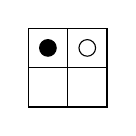
\begin{tikzpicture}[x=1cm]
			\draw (0,0)--(1,0)--(1,1)--(0,1)--cycle;
			\draw (.5,0)--(.5,.5)--(.5,1);
			\draw (0,.5)--(.5,.5)--(1,.5);
			\draw (.75,.75) circle (3pt);
			\filldraw (.25,.75) circle (3pt);
		\end{tikzpicture}
		\caption{$c_{11}$}
	\end{subfigure}%
	%c12
	\begin{subfigure}[t]{.1\textwidth}
		\centering
		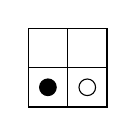
\begin{tikzpicture}[x=1cm]
			\draw (0,0)--(1,0)--(1,1)--(0,1)--cycle;
			\draw (.5,0)--(.5,.5)--(.5,1);
			\draw (0,.5)--(.5,.5)--(1,.5);
			\draw (.75,.25) circle (3pt);
			\filldraw (.25,.25) circle (3pt);
		\end{tikzpicture}
		\caption{$c_{12}$}
	\end{subfigure}
	\caption{Twelve configurations}
\end{figure}

A configuration can be transformed into other configuration according to certain rules. Specifically, we say that the configuration $c_{i}$ can be transformed into the configuration $c_{j}$ $(1 \leq i, j \leq 12, i \neq j)$ if $c_{j}$ can be obtained from $c_{i}$ by performing exactly one of the following two steps:
\begin{enumerate}[{(1)}]
\item moving one of the coins in $c_{i}$ horizontally or vertically to an unoccupied square;
\item interchanging the two coins in $c_{i}$.
\end{enumerate}
Necessarily, if $c_{i}$ can be transformed into $c_{j}$, then $c_{j}$ can be transformed into $c_{i}$. For example, $c_{2}$ can be transformed (i) into $c_{1}$ by shifting the silver coin in $c_{2}$ to the right, (ii) into $c_{4}$ by shifting the gold coin to the right or (iii) into $c_{8}$ by interchanging the two coins (see Figure 1.5).

\begin{figure}[h]
	\centering
	\begin{tikzpicture}[x=2cm, every edge/.style={draw,postaction={decorate,decoration={markings,mark=at position 1.0 with {\arrow[scale=2]{>}}}}}]
		\node[rectangle] (c2) at (1,2) [label=left:$c_{2}:$]{
			\begin{tikzpicture}[x=1cm]
				\draw (0,0)--(1,0)--(1,1)--(0,1)--cycle;
				\draw (.5,0)--(.5,.5)--(.5,1);
				\draw (0,.5)--(.5,.5)--(1,.5);
				\draw (.25,.25) circle (3pt);
				\filldraw (.25,.75) circle (3pt);
			\end{tikzpicture}		
		};
		\node[rectangle] (c1) at (0,0) [label=below:$c_{1}$]{
			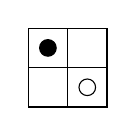
\begin{tikzpicture}[x=1cm]
				\draw (0,0)--(1,0)--(1,1)--(0,1)--cycle;
				\draw (.5,0)--(.5,.5)--(.5,1);
				\draw (0,.5)--(.5,.5)--(1,.5);
				\draw (.75,.25) circle (3pt);
				\filldraw (.25,.75) circle (3pt);
			\end{tikzpicture}
		};
		\node[rectangle] (c4) at (1,0) [label=below:$c_{4}$]{
			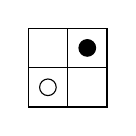
\begin{tikzpicture}[x=1cm]
				\draw (0,0)--(1,0)--(1,1)--(0,1)--cycle;
				\draw (.5,0)--(.5,.5)--(.5,1);
				\draw (0,.5)--(.5,.5)--(1,.5);
				\draw (.25,.25) circle (3pt);
				\filldraw (.75,.75) circle (3pt);
			\end{tikzpicture}
		};
		\node[rectangle] (c8) at (2,0) [label=below:$c_{8}$]{
			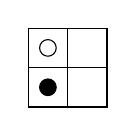
\begin{tikzpicture}[x=1cm]
				\draw (0,0)--(1,0)--(1,1)--(0,1)--cycle;
				\draw (.5,0)--(.5,.5)--(.5,1);
				\draw (0,.5)--(.5,.5)--(1,.5);
				\draw (.25,.75) circle (3pt);
				\filldraw (.25,.25) circle (3pt);
			\end{tikzpicture}
		};
		\path
			(c2) edge (c1)
			(c2) edge (c4)
			(c2) edge (c8)
		;
	\end{tikzpicture}
	\caption{Transformations of the configuration $c_{2}$}
\end{figure}

Now consider the twelve configurations shown in Figure 1.4. Some pairs $c_{i}, c_{j}$ of these configurations, where $1 \leq i, j \leq 12, i \neq j$, can be transformed into each other and some pairs cannot. This situation can also be represented by a graph $F$ where $V(F) = \{c_{1},c_{2},\ldots,c_{12}\}$ and $c_{i}c_{j}$ is an edge of $F$ if $c_{i}$ and $c_{j}$ can be transformed into each other. This graph $F$ is shown in Figure 1.6.
\end{exmp}

\begin{figure}[h]
	\[F:
	\raisebox{-.5\height}
	{
		\begin{tikzpicture}[x=1.5cm, y=1.5cm]
			\foreach \i/\j in {-1/1, -2/2, -3/3, 8/4, 7/5, 6/6, 5/7, 4/8, 3/9, 2/10, 1/11, 0/12} {
				\setcounter{Angle}{90 + \i * 360 / 12};
				\vertex (c\j) at (\theAngle:1) [label=\theAngle:$c_{\j}$]{};
			}
			\path
				(c1) edge (c2)
				(c1) edge (c3)
				(c1) edge (c7)
				(c1) edge (c11)
				(c1) edge (c12)
				(c2) edge (c4)
				(c2) edge (c8)
				(c3) edge (c4)
				(c3) edge (c9)
				(c4) edge (c5)
				(c4) edge (c6)
				(c4) edge (c10)
				(c5) edge (c7)
				(c5) edge (c11)
				(c6) edge (c7)
				(c6) edge (c12)
				(c7) edge (c8)
				(c7) edge (c9)
				(c8) edge (c10)
				(c9) edge (c10)
				(c10) edge (c11)
				(c10) edge (c12)
			;
		\end{tikzpicture}
	}\]
	\caption{Modeling transformations of twelve configurations}
\end{figure}

Let's look at a somewhat related example.

\begin{exmp}
Suppose that we have a collection of 3-letter English words, say
\begin{align*}
ACT, AIM, ARC, ARM, ART, CAR, CAT, OAR, OAT, RAT, TAR.
\end{align*}
We say that a word $W_{1}$ can be transformed into a word $W_{2}$ if $W_{2}$ can be obtained from $W_{1}$ by performing exactly one of the following two steps:
\begin{enumerate}[{(1)}]
\item interchanging two letters of $W_{1}$;
\item replacing a letter in $W_{1}$ by another letter.
\end{enumerate}
Therefore, if $W_{1}$ can be transformed into $W_{2}$, then $W_{2}$ can be transformed into $W_{1}$. This situation can be modeled by a graph $G$, where the given words are the vertices of $G$ and two vertices are adjacent in $G$ if the corresponding words can be transformed into each other. This graph is called \bf{the word graph of the set of words}. For the 11 words above, its word graph $G$ is shown in Figure 1.7.

\begin{figure}[h]
	\[G:
	\raisebox{-.5\height}
	{
		\begin{tikzpicture}[x=1.5cm, y=1.5cm]
			\vertex (AIM) at (0,1.5) [label=above:$AIM$]{};
			\vertex (ARM) at (1,1.5) [label=above:$ARM$]{};
			\vertex (ACT) at (2,0) [label=below:$ACT$]{};
			\vertex (ART) at (2,1) [label=left:$ART$]{};
			\vertex (ARC) at (2,2) [label=above:$ARC$]{};
			\vertex (CAT) at (3,0) [label=below:$CAT$]{};
			\vertex (RAT) at (3,1) [label=above:$RAT$]{};
			\vertex (OAT) at (4,.5) [label=above:$OAT$]{};
			\vertex (OAR) at (5,.5) [label=below:$OAR$]{};
			\vertex (CAR) at (6,0) [label=below:$CAR$]{};
			\vertex (TAR) at (6,1) [label=above:$TAR$]{};
			\path
				(AIM) edge (ARM)
				(ARM) edge (ART)
				(ARM) edge (ARC)
				(ACT) edge (ART)
				(ACT) edge (CAT)
				(ART) edge (ARC)
				(ART) edge (RAT)
				(CAT) edge (RAT)
				(CAT) edge (OAT)
				(CAT) edge (CAR)
				(RAT) edge (OAT)
				(RAT) edge (TAR)
				(OAT) edge (OAR)
				(OAR) edge (CAR)
				(OAR) edge (TAR)
				(CAR) edge (TAR)
			;
		\end{tikzpicture}
	}\]
	\caption{The word graph of a set of 11 words}
\end{figure}

In this case, a graph $G$ is called \bf{a word graph} if $G$ is the word graph of some set $S$ of 3-letter words. For example, the (unlabeled) graph $G$ of Figure 1.8(a) is a word graph because it is the word graph of the set $S = \{BAT, BIT, BUT, BAD, BAR, CAT, HAT\}$, as shown in Figure 1.8(b). (This idea is related to the concept of "isomorphic graphs," which will be discussed in Chapter 3.)
\end{exmp}

\begin{figure}[h]
	\centering
	\begin{subfigure}[b]{.4\textwidth}
		\[G:
		\raisebox{-.5\height}
		{
			\begin{tikzpicture}[x=1.5cm, y=1.5cm]
				\vertex (BAD) at (0,.5){};
				\vertex (BAR) at (.5,0){};
				\vertex (BIT) at (.5,1){};
				\vertex (BAT) at (1,.5){};
				\vertex (HAT) at (1.5,0){};
				\vertex (BUT) at (1.5,1){};
				\vertex (CAT) at (2,.5){};
				\path
					(BAD) edge (BAR)
					(BAD) edge (BAT)
					(BAR) edge (BAT)
					(BIT) edge (BUT)
					(BIT) edge (BAT)
					(BUT) edge (BAT)
					(HAT) edge (BAT)
					(HAT) edge (CAT)
					(CAT) edge (BAT)
				;
			\end{tikzpicture}
		}\]
		\caption{}
	\end{subfigure}%
	\begin{subfigure}[b]{.4\textwidth}
		\[\raisebox{-.5\height}
		{
			\begin{tikzpicture}[x=1.5cm, y=1.5cm]
				\vertex (BAD) at (0,.5) [label=left:$BAD$]{};
				\vertex (BAR) at (.5,0) [label=left:$BAR$]{};
				\vertex (BIT) at (.5,1) [label=left:$BIT$]{};
				\vertex (BAT) at (1,.5) [label=below:$BAT$]{};
				\vertex (HAT) at (1.5,0) [label=right:$HAT$]{};
				\vertex (BUT) at (1.5,1) [label=right:$BUT$]{};
				\vertex (CAT) at (2,.5) [label=right:$CAT$]{};
				\path
					(BAD) edge (BAR)
					(BAD) edge (BAT)
					(BAR) edge (BAT)
					(BIT) edge (BUT)
					(BIT) edge (BAT)
					(BUT) edge (BAT)
					(HAT) edge (BAT)
					(HAT) edge (CAT)
					(CAT) edge (BAT)
				;
			\end{tikzpicture}
		}\]
		\caption{}
	\end{subfigure}
	\caption{A word graph}
\end{figure}

We conclude this section with one last example.

\begin{exmp}
Figure 1.9 shows the traffic lanes at the intersection of two busy streets. When a vehicle approaches this intersection, it could be in one of the nine lanes: L1, L2, \ldots, L9.

\begin{figure}[h]
	\centering
	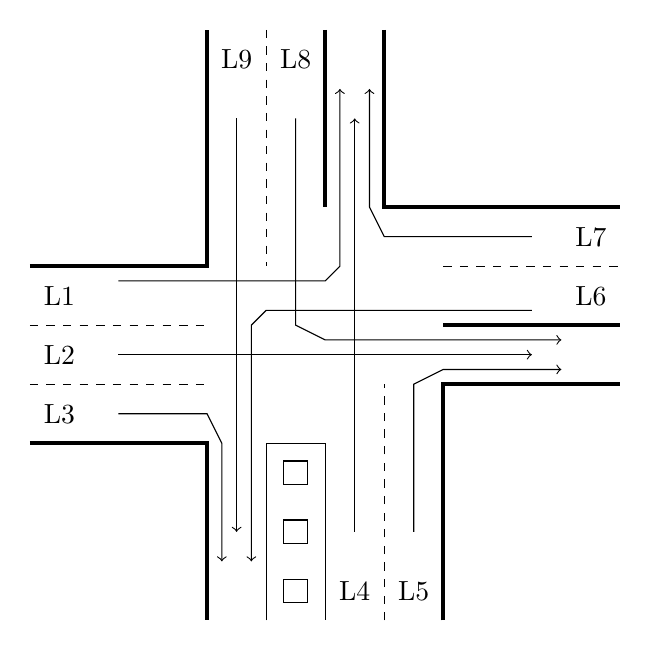
\begin{tikzpicture}[x=1.5cm,y=1.5cm,scale=.5]
		\draw[ultra thick] (0,3)--(3,3)--(3,0);
		\draw[ultra thick] (0,6)--(3,6)--(3,10);
		\draw[ultra thick] (5,10)--(5,7);
		\draw[ultra thick] (6,10)--(6,7)--(10,7);
		\draw[ultra thick] (7,5)--(10,5);
		\draw[ultra thick] (7,0)--(7,4)--(10,4);
		\draw[dashed] (0,4)--(3,4);
		\draw[dashed] (0,5)--(3,5);
		\draw[dashed] (4,10)--(4,6);
		\draw[dashed] (7,6)--(10,6);
		\draw[dashed] (6,0)--(6,4);
		\draw (4,0)--(4,3)--(5,3)--(5,0);
		\draw (4.3,.3)--(4.3,.7)--(4.7,.7)--(4.7,.3)--cycle;
		\draw (4.3,1.3)--(4.3,1.7)--(4.7,1.7)--(4.7,1.3)--cycle;
		\draw (4.3,2.3)--(4.3,2.7)--(4.7,2.7)--(4.7,2.3)--cycle;
		\draw[-{>[scale=2]}] (1.5,3.5)--(3,3.5)--(3.25,3)--(3.25,1);
		\draw[-{>[scale=2]}] (1.5,4.5)--(8.5,4.5);
		\draw[-{>[scale=2]}] (1.5,5.75)--(5,5.75)--(5.25,6)--(5.25,9);
		\draw[-{>[scale=2]}] (3.5,8.5)--(3.5,1.5);
		\draw[-{>[scale=2]}] (4.5,8.5)--(4.5,5)--(5,4.75)--(9,4.75);
		\draw[-{>[scale=2]}] (8.5,6.5)--(6,6.5)--(5.75,7)--(5.75,9);
		\draw[-{>[scale=2]}] (8.5,5.25)--(4,5.25)--(3.75,5)--(3.75,1);
		\draw[-{>[scale=2]}] (6.5,1.5)--(6.5,4)--(7,4.25)--(9,4.25);
		\draw[-{>[scale=2]}] (5.5,1.5)--(5.5,8.5);
		\node at (.5,3.5) {L3};
		\node at (.5,4.5) {L2};
		\node at (.5,5.5) {L1};
		\node at (3.5,9.5) {L9};
		\node at (4.5,9.5) {L8};
		\node at (9.5,6.5) {L7};
		\node at (9.5,5.5) {L6};
		\node at (6.5,.5) {L5};
		\node at (5.5,.5) {L4};
	\end{tikzpicture}
	\caption{Traffic lanes at street intersections}
\end{figure}

This intersection has a traffic light that informs drivers in vehicles in the various lanes when they are permitted to proceed through the intersection. To be sure, there are pairs of lanes containing vehicles that should not enter the intersection at the same time, such as L1 and L7. However, there would be no difficulty for vehicles in L1 and L5 to drive through this intersection at the same time. This situation can be represented by the graph $G$ of Figure 1.10, where $V(G)$ = \{L1,L2,\ldots,L9\} and two vertices (lanes) are joined by an edge if vehicles in these two lanes cannot safely enter the intersection at the same time, as there would be a possibility of an accident.
\end{exmp}

\begin{figure}[h]
	\[G:
	\raisebox{-.5\height}
	{
		\begin{tikzpicture}[x=1.5cm, y=1.5cm]
			\foreach \i/\j in {0/1, -1/2, -2/3, 6/4, 5/5, 4/6, 3/7, 2/8, 1/9} {
				\setcounter{Angle}{90 + \i * 360 / 9};
				\vertex (L\j) at (\theAngle:1) [label=\theAngle:$L\j$]{};
			}
			\path
				(L1) edge (L4)
				(L1) edge (L7)
				(L1) edge (L8)
				(L1) edge (L9)
				(L2) edge (L4)
				(L2) edge (L5)
				(L2) edge (L6)
				(L2) edge (L8)
				(L2) edge (L9)
				(L3) edge (L6)
				(L3) edge (L9)
				(L4) edge (L6)
				(L4) edge (L7)
				(L4) edge (L8)
				(L5) edge (L8)
				(L6) edge (L8)
				(L6) edge (L9)
			;
		\end{tikzpicture}
	}\]
	\caption{The graph $G$ in Example 1.5}
\end{figure}

What we have just seen is how five different situations can be represented by graphs. Actually, in each case, there is a set involved: (1) a set of committees, (2) a set of integers, (3) a set of configurations consisting of two coins on a $2 \times 2$ checkerboard, (4) a set of 3-letter words, (5) a set of traffic lanes at a street intersection. Certain pairs of elements in each set are related in some manner: (1) two committees have a member in common, (2) the sum or difference (in absolute value) of two integers in the set also belongs to the set, (3) two configurations can be transformed into each other according to some rule, (4) two 3-letter words can be transformed into each other by certain movements of letters, (5) cars in certain pairs of traffic lanes cannot enter the intersection at the same time. In each case, a graph $G$ is defined whose vertices are the elements of the set and two vertices of $G$ are adjacent if they are related as described above. The graph $G$ then \it{models} the given situation. Often questions concerning the situations described above arise and can be analyzed by studying the graphs that model them. We will encounter such questions throughout the text and discuss how graphs can be used to help us answer the questions.

\begin{exers}\end{exers}

\begin{exer}
What is a logical question to ask in Example 1.1? Answer this question.
\end{exer}

\begin{exer}
Create an example of your own similar to Example 1.1 with nine editors and eight committees and then draw the corresponding graph.
\end{exer}

\begin{exer}
Let $S = \{2,3,4,7,11,13\}$. Draw the graph $G$ whose vertex set is $S$ and such that $ij \in E(G)$ for $i,j \in S$ if $i+j \in S$ or $|i-j| \in S$.
\end{exer}

\begin{exer}
Let $S = \{-6,-3,0,3,6\}$. Draw the graph $G$ whose vertex set is $S$ and such that $ij \in E(G)$ for $i,j \in S$ if $i+j \in S$ or $|i-j| \in S$.
\end{exer}

\begin{exer}
Create your own set $S$ of integers and draw the graph $G$ whose vertex set is $S$ and such that $ij \in E(G)$ if $i$ and $j$ are related by some rule imposed on $i$ and $j$.
\end{exer}

\begin{exer}
Consider the twelve configurations $c_{1},c_{2},\ldots,c_{12}$ in Figure 1.4. For every two configurations $c_{i}$ and $c_{j}$, where $1 \leq i,j \leq 12, i \neq j$, it may be possible to obtain $c_{j}$ from $c_{i}$ by first shifting one of the coins in $c_{i}$ horizontally or vertically \it{and} then interchanging the two coins. Model this by a graph $F$ such that $V(F) = \{c_{1},c_{2},\ldots,c_{12}\}$ and $c_{i}c_{j}$ is an edge of $F$ if $c_{i}$ and $c_{j}$ can be transformed into each other by this 2-step process.
\end{exer}

\begin{exer}
Following Example 1.4,
\begin{enumerate}[{(a)}]
\item give an example of ten 3-letter words, none of which are mentioned in Example 1.4 and whose corresponding word graph has at least six edges. Draw this graph.
\item give a set of five 3-letter words whose word graph is shown in Figure 1.11 (with the vertices appropriately labeled).
\begin{figure}[h]
	\centering
	\begin{tikzpicture}[x=1.5cm, y=1.5cm]
		\foreach \i in {1,2,3,4,5} {
			\vertex (\i) at (\i,0){};
		}
		\path
			(1) edge (2)
			(2) edge (3)
			(3) edge (4)
			(4) edge (5)
		;
	\end{tikzpicture}
	\caption{The graph in Exercise 1.7(b)}
\end{figure}
\item give a set of five 3-letter words whose word graph is shown in Figure 1.12 (with the vertices appropriately labeled).
\begin{figure}[h]
	\centering
	\begin{tikzpicture}[x=1.5cm, y=1.5cm]
		\foreach \i in {1,2,3,4,5} {
			\setcounter{Angle}{90 + \i * 360 / 5};
			\vertex (\i) at (\theAngle:.75){};
		}
		\path
			(1) edge (2)
			(1) edge (5)
			(2) edge (3)
			(3) edge (4)
			(4) edge (5)
		;
	\end{tikzpicture}
	\caption{The graph in Exercise 1.7(c)}
\end{figure}
\end{enumerate}
\end{exer}

\begin{exer}
Let $S$ be a finite set of 3-letter and/or 4-letter words. In this case, the word graph $G(S)$ of $S$ is that graph whose vertex set is $S$ and such that two vertices (words) $w_{1}$ and $w_{2}$ are adjacent if either (1) or (2) below occurs:
\begin{enumerate}[{(1)}]
\item one of the words can be obtained from the other by replacing one letter by another letter,
\item $w_{1}$ is a 3-letter word and $w_{2}$ is a 4-letter word and $w_{2}$ can be obtained from $w_{1}$ by the insertion of a single letter (anywhere, including the beginning or the end) into $w_{1}$.
\end{enumerate}
\begin{enumerate}[{(a)}]
\item Find six sets $S_{1},S_{2},\ldots,S_{6}$ of 3-letter and/or 4-letter words so that for each integer $i$ $(1 \leq i \leq 6)$ the graph $G_{i}$ of Figure 1.13 is the word graph of $S_{i}$.
\item For another graph $H$ (of your choice), determine whether $H$ is a word graph of some set.
\end{enumerate}

\begin{figure}[h]
	\centering
	\captionsetup[subfigure]{labelformat=empty}
	\begin{subfigure}[b]{.1\textwidth}
		\centering
		\begin{tikzpicture}[x=1.5cm]
			\foreach \i in {0,1,2,3} {
				\vertex (\i) at (0,\i * .5){};
			}
			\path
				(0) edge (1)
				(1) edge (2)
				(2) edge (3)
			;
		\end{tikzpicture}
		\caption{$G_{1}$}
	\end{subfigure}%
	\begin{subfigure}[b]{.1\textwidth}
		\centering
		\begin{tikzpicture}[x=1.5cm]
			\foreach \i in {0,1,2} {
				\setcounter{Angle}{270 + \i * 360 / 3};
				\vertex (\i) at (\theAngle:.5){};
			}
			\vertex (3) at (0,0){};
			\path
				(3) edge (0)
				(3) edge (1)
				(3) edge (2)
			;
		\end{tikzpicture}
		\caption{$G_{2}$}
	\end{subfigure}%
	\begin{subfigure}[b]{.1\textwidth}
		\centering
		\begin{tikzpicture}[x=1.5cm]
			\foreach \i in {0,1,2} {
				\setcounter{Angle}{270 + \i * 360 / 3};
				\vertex (\i) at (\theAngle:.5){};
			}
			\vertex (3) at (0,0){};
			\path
				(3) edge (0)
				(3) edge (1)
				(3) edge (2)
				(1) edge (2)
			;
		\end{tikzpicture}
		\caption{$G_{3}$}
	\end{subfigure}%
	\begin{subfigure}[b]{.1\textwidth}
		\centering
		\begin{tikzpicture}[x=1.5cm]
			\foreach \i in {0,1,2,3} {
				\setcounter{Angle}{45 + \i * 360 / 4};
				\vertex (\i) at (\theAngle:.5){};
			}
			\path
				(0) edge (1)
				(0) edge (3)
				(1) edge (2)
				(2) edge (3)
			;
		\end{tikzpicture}
		\caption{$G_{4}$}
	\end{subfigure}%
	\begin{subfigure}[b]{.1\textwidth}
		\centering
		\begin{tikzpicture}[x=1.5cm]
			\foreach \i in {0,1,2,3} {
				\setcounter{Angle}{45 + \i * 360 / 4};
				\vertex (\i) at (\theAngle:.5){};
			}
			\path
				(0) edge (1)
				(0) edge (3)
				(1) edge (2)
				(1) edge (3)
				(2) edge (3)
			;
		\end{tikzpicture}
		\caption{$G_{5}$}
	\end{subfigure}%
	\begin{subfigure}[b]{.1\textwidth}
		\centering
		\begin{tikzpicture}[x=1.5cm]
			\foreach \i in {0,1,2,3} {
				\setcounter{Angle}{45 + \i * 360 / 4};
				\vertex (\i) at (\theAngle:.5){};
			}
			\path
				(0) edge (1)
				(0) edge (2)
				(0) edge (3)
				(1) edge (2)
				(1) edge (3)
				(2) edge (3)
			;
		\end{tikzpicture}
		\caption{$G_{6}$}
	\end{subfigure}
	\caption{The graphs for Exercise 1.8(a)}
\end{figure}
\end{exer}

\begin{exer}
Define a word graph differently from the word graphs defined in Example 1.4 and Exercise 1.8 and illustrate your definition.
\end{exer}

\begin{exer}
\begin{figure}[h]
	\centering
	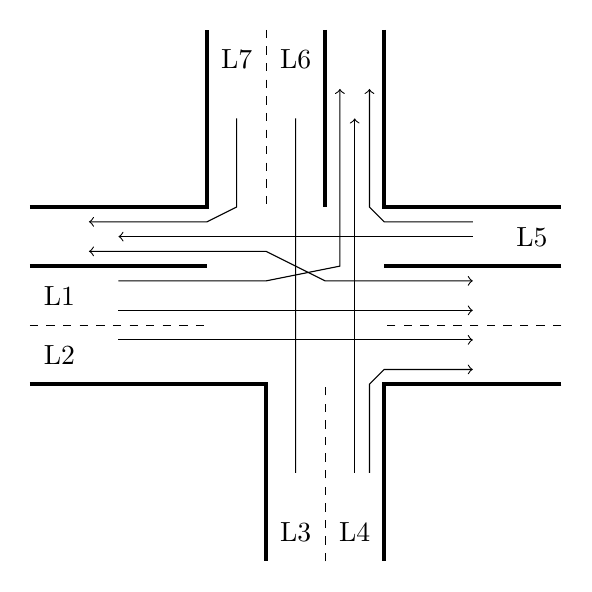
\begin{tikzpicture}[x=1.5cm,y=1.5cm,scale=.5]
		\draw[ultra thick] (0,3)--(4,3)--(4,0);
		\draw[ultra thick] (0,5)--(3,5);
		\draw[ultra thick] (0,6)--(3,6)--(3,9);
		\draw[ultra thick] (5,9)--(5,6);
		\draw[ultra thick] (6,9)--(6,6)--(9,6);
		\draw[ultra thick] (9,5)--(6,5);
		\draw[ultra thick] (9,3)--(6,3)--(6,0);
		\draw[dashed] (0,4)--(3,4);
		\draw[dashed] (4,9)--(4,6);
		\draw[dashed] (9,4)--(6,4);
		\draw[dashed] (5,0)--(5,3);
		\draw[-{>[scale=2]}] (1.5,3.75)--(7.5,3.75);
		\draw[-{>[scale=2]}] (1.5,4.25)--(7.5,4.25);
		\draw[-{>[scale=2]}] (1.5,4.75)--(4,4.75)--(5.25,5)--(5.25,8);
		\draw[-{>[scale=2]}] (3.5,7.5)--(3.5,6)--(3,5.75)--(1,5.75);
		\draw[-{>[scale=2]}] (4.5,7.5)--(4.5,5)--(5,4.75)--(7.5,4.75);
		\draw[-{>[scale=2]}] (7.5,5.75)--(6,5.75)--(5.75,6)--(5.75,8);
		\draw[-{>[scale=2]}] (7.5,5.5)--(1.5,5.5);
		\draw[-{>[scale=2]}] (5.75,1.5)--(5.75,3)--(6,3.25)--(7.5,3.25);
		\draw[-{>[scale=2]}] (5.5,1.5)--(5.5,7.5);
		\draw[-{>[scale=2]}] (4.5,1.5)--(4.5,5)--(4,5.25)--(1,5.25);
		\node at (.5,3.5) {L2};
		\node at (.5,4.5) {L1};
		\node at (3.5,8.5) {L7};
		\node at (4.5,8.5) {L6};
		\node at (8.5,5.5) {L5};
		\node at (5.5,.5) {L4};
		\node at (4.5,.5) {L3};
	\end{tikzpicture}
	\caption{Traffic lanes at a street intersection in Exercise 1.10}
\end{figure}

Figure 1.14 illustrates the traffic lanes at the intersection of two streets. When a vehicle approaches this intersection, it could be in one of the seven lanes: L1, L2, \ldots, L7. Draw a graph $G$ that models this situation, where $V(G)$ = \{L1,L2,\ldots,L7\} and wher two vertices are joined by an edge if vehicles in these two lanes cannot safely enter this intersection at the same time.
\end{exer}